%%%%%%%%%%%%%%%%%%%%%%%%%%%%%%%%%%%%%%%%%%%%%%%%%%%%%%%%%%%%%%%%%%%%%%%%%%
% PART: SLIDE n°3
\frame{
\frametitle{Tracers \textit{vs} Inertial Particles}
\begin{textblock*}{45mm}[0,0](-4mm,0mm)
   	\footnotesize{Tracers behave as fluid particles}\\[2pt]
	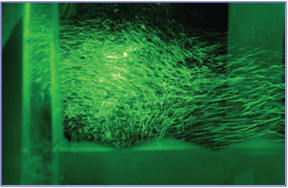
\includegraphics[width=\textwidth]{tracer.png}
\end{textblock*}
\begin{textblock*}{30mm}[0,0](5mm,30mm)
	\small{\textcolor{white}{PIV, LDV, PTV}}
\end{textblock*}

\begin{textblock*}{60mm}[0,0](51mm,0mm)
	\footnotesize{Inertial particles do not follow the flow}\\[2pt]
	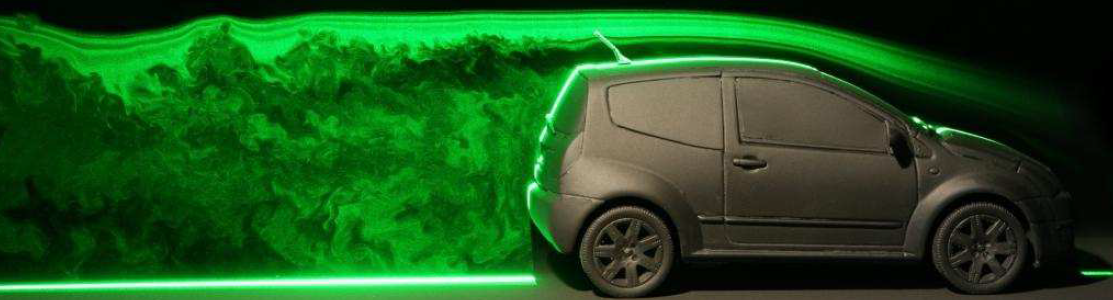
\includegraphics[clip,trim=90 0 70 0,height=22mm]{sillage_voiture.png}
\end{textblock*}
\begin{textblock*}{80mm}[0,0](82mm,28mm)
	\tiny{Grandemange et al, ENSTA 2016}
\end{textblock*}
%
\begin{textblock*}{30mm}[0,0](0mm,40mm)
\onslide<2->{
	\footnotesize{Cluster formation}\\[2pt]
	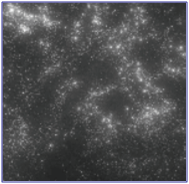
\includegraphics[width=30mm]{inertial.png}
}
\end{textblock*}
\begin{textblock*}{30mm}[0,0](4mm,74mm)
\onslide<2->{
	\tiny{Wood \textit{et al.},	\textit{IJMF}, 31, \textbf{2005}}
}
\end{textblock*}
%
\begin{textblock*}{30mm}[0,0](40mm,40mm)
\onslide<3->{
	\footnotesize{Settling alteration}\\[2pt]
	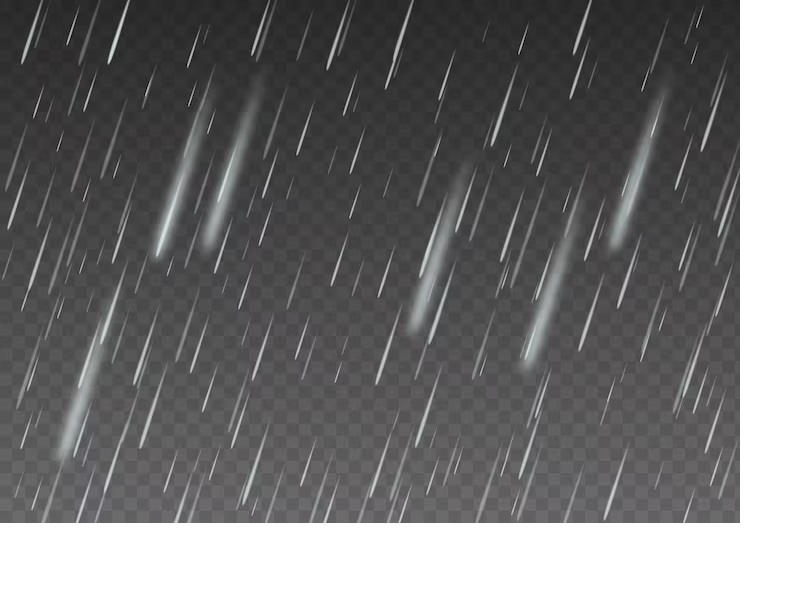
\includegraphics[clip,trim=60 0 60 0,width=30mm]{rain_enhance.jpg}
}
\end{textblock*}
\begin{textblock*}{30mm}[0,0](55mm,70mm)
\onslide<3->{
	\tiny{Artist view}
}
\end{textblock*}
%
\begin{textblock*}{30mm}[0,0](80mm,40mm)
\onslide<4->{
	\footnotesize{Collision alteration}\\[2pt]
	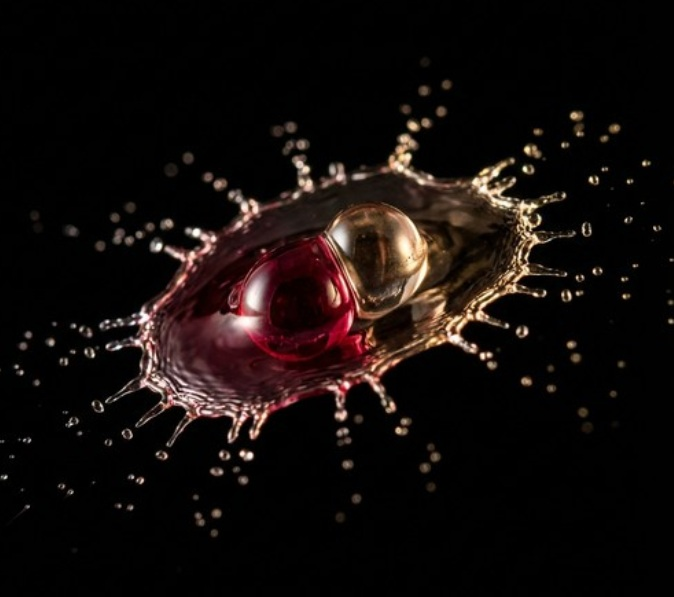
\includegraphics[width=30mm]{collision.jpg}
}
\end{textblock*}
\begin{textblock*}{30mm}[0,0](95mm,71mm)
\onslide<4->{
	\tiny{Artist view}
}
\end{textblock*}
%
\begin{textblock*}{30mm}[0,0](52mm,77mm)
\onslide<5->{
	\footnotesize{Flow modulation, Dispersion\ldots}
}
\end{textblock*}

%
}